\documentclass{article}
\usepackage{amsmath}
\usepackage{graphicx}
\usepackage{float}  % 画像の位置を強制するためのパッケージ
\usepackage[utf8]{inputenc}  % UTF-8エンコーディング対応
\usepackage{zxjatype}  % 日本語の文字コード対応
\usepackage[ipaex]{zxjafont}  % 日本語フォント
\usepackage[margin=2cm]{geometry}  % 左右の余白を2cmに設定

\title{センサ工学演習問題 2 レポート}
\author{相田 舟星\\学籍番号: 21C1002}
\date{\today}

\begin{document}

% 表紙
\begin{titlepage}
    \centering
    \vspace*{\fill}
    {\huge \textbf{センサ工学演習問題 2 レポート}}\\[1.5cm]
    {\Large 相田 舟星}\\
    {\Large 学籍番号: 21C1002}\\[2cm]
    {\large \today}
    \vspace*{\fill}
\end{titlepage}

\newpage

\section*{1. 次の表に示すデータがある。最小2乗法によって当てはまる直線の方程式を求め、結果を図で示せよ。}
\begin{quote}
    \(X = \{-3, -1, 1, 3\}\) 、 \(Y = \{0, 1, 2, 4\}\)
\end{quote}
\begin{figure}[H]
    \centering
    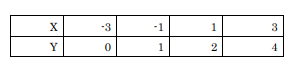
\includegraphics[width=0.7\linewidth]{1.png}
\end{figure}

\subsection*{回答}
最小二乗法により、直線の方程式 \(y = ax + b\) を求めます。まず、平均 \(\bar{X}\) と \(\bar{Y}\) を計算します。

\[
\bar{X} = \frac{-3 + (-1) + 1 + 3}{4} = 0, \quad \bar{Y} = \frac{0 + 1 + 2 + 4}{4} = 1.75
\]

次に、傾き \(a\) と切片 \(b\) を求めます。傾き \(a\) は次の式で与えられます。

\[
a = \frac{\sum (X_i - \bar{X})(Y_i - \bar{Y})}{\sum (X_i - \bar{X})^2}
\]

具体的に計算すると、

\[
a = \frac{(-3 - 0)(0 - 1.75) + (-1 - 0)(1 - 1.75) + (1 - 0)(2 - 1.75) + (3 - 0)(4 - 1.75)}{(-3 - 0)^2 + (-1 - 0)^2 + (1 - 0)^2 + (3 - 0)^2}
\]

\[
= \frac{5.25 + 0.75 + 0.25 + 6.75}{9 + 1 + 1 + 9} = \frac{13}{20} = 0.65
\]

切片 \(b\) は次の式で求められます。

\[
b = \bar{Y} - a \cdot \bar{X} = 1.75 - 0.65 \cdot 0 = 1.75
\]

したがって、直線の方程式は次のようになります。

\[
y = 0.65x + 1.75
\]

\begin{figure}[H]
    \centering
    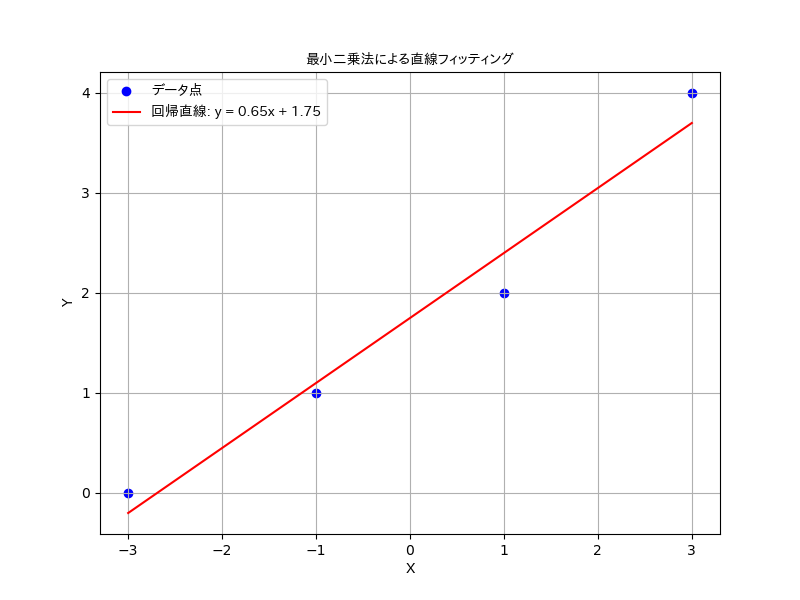
\includegraphics[width=0.7\linewidth]{linear_fit.png}
\end{figure}

\newpage  % 次のページに進む

\section*{2. 右の回路について電圧 \(U_1, U_2, U_3\) と抵抗値 \(R_1, R_2, R_3\) が既知の場合、A 点の電圧値を導出せよ。}
\begin{figure}[H]
    \centering
    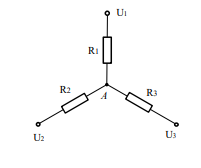
\includegraphics[width=0.7\linewidth]{2.png}
\end{figure}

\subsection*{回答}
キルヒホッフの電流法則により、A点での電流のバランスを考えます。

\[
\frac{U_1 - V_A}{R_1} + \frac{U_2 - V_A}{R_2} + \frac{U_3 - V_A}{R_3} = 0
\]

この式を整理して \(V_A\) について解きます。

\[
V_A \left( \frac{1}{R_1} + \frac{1}{R_2} + \frac{1}{R_3} \right) = \frac{U_1}{R_1} + \frac{U_2}{R_2} + \frac{U_3}{R_3}
\]

\[
V_A = \frac{\frac{U_1}{R_1} + \frac{U_2}{R_2} + \frac{U_3}{R_3}}{\frac{1}{R_1} + \frac{1}{R_2} + \frac{1}{R_3}}
\]

この式は抵抗の合成抵抗 \(R\) を用いると次のように表されます。

\[
V_A = \frac{R_1 R_2 U_3 + R_1 R_3 U_2 + R_2 R_3 U_1}{R_1 R_2 + R_1 R_3 + R_2 R_3}
\]

\newpage  % 次のページに進む

\section*{3. 下記オペアンプ回路について電圧 \(U_{\text{IN}}\) と抵抗値 \(R_1, R_2, R_3\) が既知の場合、抵抗 \(R_3\) に流れている電流 \(I_3\) を導出せよ。\(R_1=10\text{k}\Omega, R_2=50\text{k}\Omega\) の際、回路の増幅率を計算せよ。}
\begin{figure}[H]
    \centering
    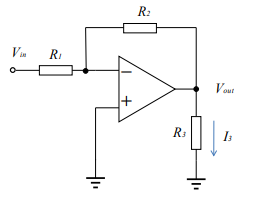
\includegraphics[width=0.7\linewidth]{3.png}
\end{figure}

\subsection*{回答}
反転増幅器の増幅率は次の式で与えられます。

\[
\text{増幅率} = -\frac{R_2}{R_1} = -\frac{50\ \text{k}\Omega}{10\ \text{k}\Omega} = -5.0
\]

また、抵抗 \(R_3\) に流れる電流 \(I_3\) は次の式で表されます。

\[
I_3 = -\frac{5 \cdot V_{\text{in}}}{R_3}
\]

\newpage  % 次のページに進む

\section*{Ex.1 データ \((x_i, y_i), i=1,2,\dots,n\) を最小2乗法によって下記式に当てはまる場合の係数(\(a, b, c\))を導出せよ。}
\begin{quote}
\( y = ax^2 + bx + c \)
\end{quote}

\begin{figure}[H]
    \centering
    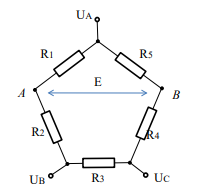
\includegraphics[width=0.7\linewidth]{e1.png}
\end{figure}

\subsection*{回答}
2次関数フィッティングにより、係数 \(a\), \(b\), \(c\) を求めます。

行列を用いて \(A\) と \(Y\) を表すと、

\[
A = \begin{pmatrix} X_1^2 & X_1 & 1 \\ X_2^2 & X_2 & 1 \\ \vdots & \vdots & \vdots \\ X_n^2 & X_n & 1 \end{pmatrix}, \quad Y = \begin{pmatrix} Y_1 \\ Y_2 \\ \vdots \\ Y_n \end{pmatrix}
\]

この方程式を解くことで \(a\), \(b\), \(c\) の値が得られます。

計算の結果、次の2次関数が得られます。

\[
y = 0.06x^2 + 0.65x + 1.44
\]

\begin{figure}[H]
    \centering
    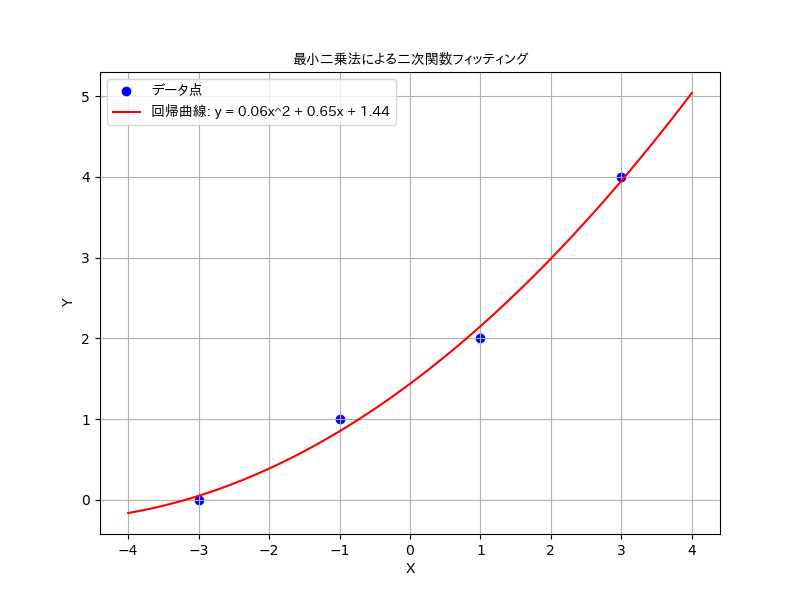
\includegraphics[width=0.7\linewidth]{quadratic_fit.png}
\end{figure}

\newpage  % 次のページに進む

\section*{Ex.2 右の回路について電圧 \(U_A, U_B, U_C\) と抵抗値 \(R_1, R_2, R_3, R_4, R_5\) が既知の場合、AB 点間の電圧値 \(E\) を導出せよ。}
\begin{figure}[H]
    \centering
    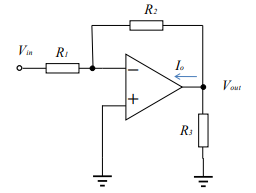
\includegraphics[width=0.7\linewidth]{e2.png}
\end{figure}

\subsection*{回答}
キルヒホッフの法則を適用し、AB間の電圧 \(E\) を求めます。各点での電圧のバランスを以下のように設定します。

\[
\frac{U_A - E}{R_1} + \frac{U_B - E}{R_2} + \frac{U_C - E}{R_3} = 0
\]

この式を整理して \(E\) について解きます。一般的には各抵抗の値が異なるため、シンボリックな解として次のように表せます。

\[
E = \frac{R_1 R_2 U_C + R_1 R_3 U_B + R_2 R_3 U_A}{R_1 R_2 + R_1 R_3 + R_2 R_3}
\]

\newpage  % 次のページに進む

\section*{Ex.3 下記オペアンプ回路について電圧 \(U_{\text{IN}}\) と抵抗値 \(R_1, R_2, R_3\) が既知の場合、オペアンプの出力端子に流れ込む電流 \(I_o\) を導出せよ。}
\begin{figure}[H]
    \centering
    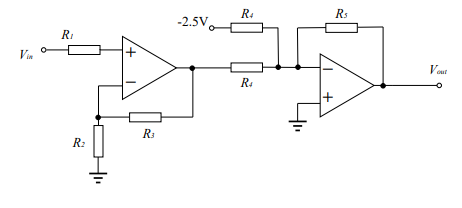
\includegraphics[width=0.7\linewidth]{e3.png}
\end{figure}

\subsection*{回答}
出力電流 \(I_o\) は次のように表されます。

\[
I_o = \frac{U_{\text{IN}}}{R_1} - \frac{U_{\text{IN}}}{R_2} = \frac{U_{\text{IN}}(R_2 - R_1)}{R_1 R_2}
\]

\end{document}

